% Template from Usenix
\documentclass[letterpaper,twocolumn,10pt]{article}
\usepackage{usenix,epsfig,endnotes}
\usepackage{graphicx}

\begin{document}

% Don't output date
\date{}

% Title
\title{\Large \textbf{
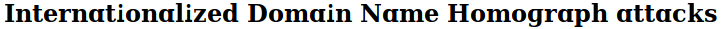
\includegraphics[height=\baselineskip]{title} \\
Project Proposal } \\ \vspace{0.025 in} \large \normalfont
CSE 227: Computer Security - Spring 2017 \\ \textit{
University of California San Diego
}}

% Authors
\author{
{\rm Chen Lai}\\
\normalfont{\texttt{chl588@ucsd.edu}}
\and
{\rm Zhongrong Jian}\\
\normalfont{\texttt{zhjian@ucsd.edu}}
\and
{\rm Juan Sidrach}\\
\normalfont{\texttt{jsidrach@ucsd.edu}}
}

\maketitle

\section{What}

- Explain the attack
  - When/how were IDN introduced
  - Homograph letters
  - How to use this to the attackers advantage

Domain name were designed to support ASCII character. Internationalized domain name(IDN) was proposed in December 1996 by Martin Dürst for the purpose of letting non-English speaking people use Internet without restriction[1]. The solution is to implement unicode mapping every character in different language to a unique number. Homograph letters, however, could be a potential vulnerability. For example, Cyrillic letter 'a' can look identical to Latin letter 'a'. Attackers can use the website "www.apple.com" where 'a' actually is a Cyrillic letter to attack users. In some other language, like Chinese, there exists many homographs between traditional Chinese and simplified Chinese.

- Research
  - On websites
    - Top 500 Alexa Websites
    - Try all possible variations
    - Classify: 404, redirect (legitimate), malicious, unrelated
    - Evaluation
  - On browsers
    - % Affected, version affected
    - Screenshots before/after CVE (url bar, hover link)
    - Other possible policies: why they may work or they won't
      - Maybe domain providers should not allow IDNs close to real names?
      - Whitelist/blacklist

In terms of URL variations, We will mainly focus our research on Top 500 Alexa websites, replacing the domain name with all possible variations. By checking the status code of return pages, we can classify the websites into different categories: page not found(404), redirection to legitimate url, malicious variations and unrelated variations. We will evaluate the impact of this vulnerability based on the percentage of malicious variations of the websites and potential impact based on the percentage of pages with 404. On the other hand, browser plays an important role in defending against IDN homograph attack. In this project, the exposure to this vulnerability of different versions of the major browsers will be studied. We will discuss about the solutions given by these companies and how effective those solutions are along with some screenshots of them before and after the CVE is disclosed. In addition, we will also take a look at some other policies, for example, whitelist and blacklist, and analyze the possible disadvantages.

- Conclusion
  - Impact of the vulnerability based on empirical data and % of users still vulnerable
  - Possible solution for this vulnerability. How does company solve this problem.

At the end of this project, we will have an evaluation of the current impact of the vulnerability based on the empirical data so that we can have an idea of the potential impact and the percentage of users involved.

\section{Why}
- Relatively new CVE discovered because this (https://bugs.chromium.org/p/chromium/issues/detail?id=683314)
- How something beneficial for the users IDN could be turned against them
- Hard for regular users to distinguish between real/fake sites
- Easy to collect data to evaluate impact

This CVE was recently disclosed and few relevant researches have been done. It's interesting to find how internationalized domain name which was designed to be beneficial is utilized by malicious user and turn against regular users' back. It's also fairly difficult for regular users to distinguish between legitimate websites and the variant ones so we are hoping to find out how browser protect regular users from this vulnerability after its disclosure. Moreover, the impact of this CVE can be evaluated statistically and it is easy to collect data.

\section{Potential Issues}
- The potential impact, it may be actually really low
- If we will find not legitimate sites by substitution (sample size may be low)
- If there are a lot of illegitime sites, we would need to check manually if they are just a redirect or a scam, maybe we will need to find an automatic way

There are some potential issues and limitations on this project. The potential or the real impact could be actually negligible. Since we are only collecting data from top 500 Alexa websites which makes the sample size so small that we may find very few legitimate sites by substitution. Additionally, we would need to check manually the categories the illegitimate websites belongs to till we find a way to automatize the process. 

\section{Resources}
Resources
- We believe for the TOP500 sites + variations of each one we can check it with our own computers/crawlers, same for different browsers


\end{document}
